\section{Search strategy and simulation}
\label{sec:strategyandsimulation}


Our proposed analysis strategy utilizes single-$\lq$ (i.e.\ $\mathrm{p}\,\mathrm{p}\to \tau\,\lq$), double-$\lq$ (i.e.\ $\mathrm{p}\,\mathrm{p}\to \lq\,\lq$), and non-resonant $\lq$ production (i.e.\ $\mathrm{p}\,\mathrm{p}\to \tau\tau$) as shown in Figure~\ref{fig:feynmp-prod-channels}. At leading order in $\alpha_s$, since we focus on  $U_1\to \bq\,\tau$ decays, the s$\lq$ process results in the $\textrm{b}\tau\tau$ mode, the d$\lq$ process results in the $\textrm{bb}\tau\tau$ mode, and the non-res process results in the $\tau\tau$ mode. Therefore, in all cases we obtain two $\tau$ leptons, with either 0, 1, or 2 b jets. The $\tau$ leptons decay to hadrons ($\tau_{\textrm{h}}$) or semi-leptonically to electrons or muons ($\tau_{\ell}$, $\ell = \textrm{e}$ or $\mu$). To this end, we study six final states: $\tau_{\mathrm h} \tau_{\mathrm{h}/\ell}$, $\bq\,\tau_{\mathrm h} \tau_{\mathrm{h}/\ell}$, and $\bq \bq\,\tau_{\mathrm h} \tau_{\mathrm{h}/\ell}$, which can be naively associated to non-res, s$\lq$ and d$\lq$ production, respectively.
Nevertheless, experimentally it is possible for $\bq$ jets to not be properly identified or reconstructed, leading, for instance, to a fraction of d$\lq$ signal events falling into the $\bq\,\tau_{\mathrm h} \tau_{\mathrm{h}/\ell}$ and $\tau_{\mathrm h}\tau_{\mathrm{h}/\ell}$ categories. Similarly, soft jets can fake $\bq$ jets, such that non-res processes can contribute to the $\bq\,\tau_{\mathrm h} \tau_{\mathrm{h}/\ell}$ and $\bq\bq\,\tau_{\mathrm h} \tau_{\mathrm{h}/\ell}$ final states. This kind of signal loss and mixing is taken into account in our analysis\footnote{Note that further signal mixing can also occur at the event generation level by including terms at larger order in $\alpha_s$. For example, in the non-res diagram in Figure~\ref{fig:feynmp-prod-channels}, one of the initial $\bq$ could come from a $g\to \bq\bar{\bq}$ splitting, leading to non resonant production of $\bq\,\tau_{\mathrm h} \tau_{\mathrm{h}/\ell}$. Simulating and studying the role of such NLO contributions is outside the scope of this work.}.

The contributions of signal and background events are estimated using Monte Carlo (MC) simulations. We implemented the $U_1$ model from~\cite{Baker:2019sli}, adjusted to describe the lagrangian in Equations~\eqref{eq:BasicLagrangian} and ~\eqref{eq:BasicLagrangianZp}, using \texttt{FeynRules} (v2.3.43) ~\cite{Christensen:2008py,Alloul:2013bka}. The branching ratios and cross-sections have been calculated using \texttt{MadGraph5\_aMC} (v3.1.0) \cite{Alwall:2014bza, Alwall:2014hca}, the latter at leading order in $\alpha_s$. The corresponding samples are generated considering $\mathrm{p}\,\mathrm{p}$ collisions at  $\sqrt{s}=13 \tev$ and $\sqrt{s}=13.6 \tev$.  All samples are generated using the NNPDF3.0 NLO~\cite{NNPDF:2014otw} set for parton distribution functions (PDFs) and using the full amplitude square SDE strategy for the phase-space optimization due to strong interference effects with the $\zb'$ boson. Parton level events are then interfaced with the \texttt{PYTHIA} (v8.2.44)~\cite{Sjostrand:2014zea} package to include parton fragmentation and hadronization processes, while \texttt{DELPHES} (v3.4.2)~\cite{deFavereau:2013fsa} is used to simulate detector effects, using the input card for the CMS detector geometric configurations, and for the performance of particle reconstruction and identification.

At parton level, jets and leptons are required to have a minimum transverse momentum ($\pt$) of $20 \gev$, while $\bq$ jets are required to have a minimum $\pt$ of $30 \gev$. Additionally, we constrain the pseudorapidity ($\eta$) to $|\eta| < 2.5$ for $\bq$ jets and leptons, and $|\eta| < 5.0$ for jets. The production cross-sections shown in the bottom panel of Figures~\ref{fig:branching_ratios} and~\ref{fig:xsinterference} are obtained with the aforementioned selection criteria. 

\begin{table}[t]
    \begin{tabular}{|c|cccccc|}
    \hline
    \multirow{2}{*}{\textbf{Variable}} & \multicolumn{6}{c|}{\textbf{Threshold}} \bigstrut\\ 
    \cline{2-7} 
                                      & \multicolumn{1}{c|}{$\tau_{h} \tau_{h}$} & \multicolumn{1}{c|}{$\bq \tau_{h} \tau_{h}$} & \multicolumn{1}{c|}{$\bq \bq \tau_{h} \tau_{h}$} & \multicolumn{1}{c|}{$\tau_{h} \tau_{\ell}$} & \multicolumn{1}{c|}{$\bq \tau_{h} \tau_{\ell}$} & $\bq \bq \tau_{h} \tau_{\ell}$ \bigstrut\\ \hline \hline


    $N(\bq)$                             & \multicolumn{1}{c|}{= 0} & \multicolumn{1}{c|}{= 1} & \multicolumn{1}{c|}{$\geq 2$} & \multicolumn{1}{c|}{= 0}& \multicolumn{1}{c|}{= 1} & $\geq 2$ \bigstrut\\ \hline
    $\pt(\bq)$                         & \multicolumn{1}{c|}{-} & \multicolumn{2}{c|}{$\geq 30 \gev$ } & \multicolumn{1}{c|}{-} & \multicolumn{2}{c|}{$\geq 30 \gev$ } \bigstrut\\ \hline
    $|\eta(\bq)|$                        & \multicolumn{1}{c|}{-} &\multicolumn{2}{c|}{$\leq 2.4$} & \multicolumn{1}{c|}{-} &\multicolumn{2}{c|}{$\leq 2.4$} \bigstrut\\ \hline
                                      
    $N (\ell)$                         & \multicolumn{3}{c|}{= 0}  & \multicolumn{3}{c|}{= 1} \bigstrut\\ \hline
    $\pt(\el)$                         & \multicolumn{3}{c|}{-} & \multicolumn{3}{c|}{$\geq 35 \gev$} \bigstrut\\ \hline
    $\pt(\mu)$                       & \multicolumn{3}{c|}{-} & \multicolumn{3}{c|}{$\geq 30 \gev$} \bigstrut\\ \hline
    $|\eta(\ell)|$                     & \multicolumn{3}{c|}{-} & \multicolumn{3}{c|}{$\leq 2.4$} \bigstrut\\ \hline

    $N(\tau_{h})$                      & \multicolumn{3}{c|}{ $= 2$} & \multicolumn{3}{c|}{= 1} \bigstrut\\ \hline
    $\pt(\tau_h)$                    & \multicolumn{6}{c|}{$\geq 50$ GeV} \bigstrut\\ \hline
    $|\eta(\tau_h)|$                   & \multicolumn{6}{c|}{$\leq 2.3$} \bigstrut\\ \hline
    $\Delta R(p_{i}, p_{j})$           & \multicolumn{6}{c|}{$\geq 0.3$} \bigstrut\\ \hline

    \end{tabular}

    \caption{Preliminary event selection criteria used to filter events before feeding them to the BDT algorithm. A $\Delta R(p_{i}, p_{j}) > 0.3$ requirement is imposed between all pairs of reconstructed particle candidates $p_{i}, p_{j}$. 
    }
    \label{table:selection_channels}
\end{table}
Table~\ref{table:selection_channels} shows the preliminary event selection criteria for each channel at analysis level. The channels are divided based on the multiplicity of $\bq$ jets, $N(\bq)$, number of light leptons, $N(\ell)$, number of hadronic tau leptons, $N(\tau_{\mathrm h})$, and kinematic criteria based on $\eta$, $\pt$ and spatial separation of particles in the detector volume $(\Delta R = \sqrt{(\Delta \eta)^{2} + (\Delta \phi)^{2}})$. The minimum $\pt$ thresholds for leptons are chosen  following references~\cite{CMS:2020wzx, CMS:2022goy, ATLAS:2021oiz}, based on experimental constrains associated to trigger performance. Following reference~\cite{CMS_BTV2016}, we use a flat identification efficiency for $\bq$ jets of 70\% across the entire $\pt$ spectrum with misidentification rate of 1\%. These values correspond with the  ``medium working point'' of the CMS algorithm to identify $\bq$ jets, known as DeepCSV. We also explored the ``Loose'' (``Tight'') working point using an efficiency of 85\% (45\%) and mis-identification rate of 10\% (0.1\%). The  ``medium working point'' was selected as it gives the best signal significance for the analysis. 

For the performance of $\tau_{\textrm{h}}$ identification in DELPHES, we consider the latest technique described in~\cite{CMS_DeepTau}, which is based on a deep neural network (i.e. DeepTau) that combines variables related to isolation and $\tau$-lepton lifetime as input to identify different $\tau_{\textrm{h}}$ decay modes. Following~\cite{CMS_DeepTau}, we consider three possible DeepTau ``working points'': (i) the ``Medium'' working point of the algorithm, which gives a 70\% $\tau_{\textrm{h}}$-tagging efficiency and 0.5\% light-quark and gluon jet mis-identification rate; (ii) the ``Tight'' working point, which gives a 60\% $\tau_{\textrm{h}}$-tagging efficiency and 0.2\% light-quark and gluon jet mis-identification rate; and (iii) the ``VTight'' working point, which gives a 50\% $\tau_{\textrm{h}}$-tagging efficiency and 0.1\% light-quark and gluon jet mis-identification rate. Similar to the choice of $\textrm{b}$-tagging working point, the choice of $\tau_{\textrm{h}}$-tagging working point is determined through an optimization process which maximizes discovery reach. The ``Medium'' working point was ultimately shown to provide the best sensitivity and therefore chosen for this study. For muons (electrons), the assumed identification efficiency is 95\% (85\%), with a 0.3\% (0.6\%) mis-identification rate~\cite{CMS-PAS-FTR-13-014,CMS_MUON_17001,CMS_EGM_17001}.

After applying the preliminary selection criteria, the primary sources of background are production of top quark pairs ($\tq\bar{ \tq}$), and single-top quark processes (single $\tq$), followed by production of vector bosons with associated jets from initial or final state radiation ($V$+jets), and pair production of vector bosons ($VV$). The number of simulated MC events used for each sample is shown in Table~\ref{table:MC_events}. 

\begin{table}[]
    \begin{tabular}{|c|c|c|c|c|c|}
    \hline
    \textbf{Sample}               & $\tq \bar{\tq}$ & single $\tq$ & $VV$       & $V+$jets   & signals \bigstrut\\ \hline \hline
    \textbf{$\mathbf{N_{events}}\times 10^{-6}$} & 24.31      & 11.50   & 32.35 & 39.45 & 0.60 \bigstrut\\ \hline
    \end{tabular}
    \caption{The number of simulated events for the signal and background samples.}
    \label{table:MC_events}
\end{table}

We use two different sets of signal samples. The first set includes various $\set{M_{U},g_{U}}$ scenarios, for two different values of $\beta_R\in \set{0,-1}$. We generate signal samples for $M_{U}$ values between 250 GeV and 5000 GeV, in steps of 250 GeV. The considered $g_{U}$ coupling values are between 0.25 and 3.5, in steps of 0.25. Although the signal cross-sections depend on both $M_{U}$ and $g_{U}$, the efficiencies of our selections only depend on $M_{U}$ (for all practical purposes) since the decay widths are relatively small compared to the mass of $M_{U}$ ($\frac{\Gamma_{U}}{M_{U}} < 5$\%), and thus more sensitive to experimental resolution. In total there are 280 $\set{M_{U},g_{U},\beta_{R}}$ scenarios simulated for this first set of signal samples, and for each of these scenarios two subsets of samples are generated, which are used separately for the training and testing of the machine learning algorithm. The second set of signal samples is used to evaluate interference effects between $\lq$s and the $\zb^{\prime}$ bosons in non-res production. Using benchmark values $g_U=1.8$ and $\beta_R=0$, we consider various $\set{M_{U},g_{\zb^{\prime}}}$ scenarios for two different $\zb^{\prime}$ mass hypotheses, $\left(M_{\zb'}/M_U\right)^2 \in \Set{\tfrac{1}{2},\tfrac{3}{2}}$. The $M_{U}$ values vary between 500 GeV and 5000 GeV, in steps of 250 GeV. The $g_{\zb^{\prime}}$ coupling values are between 0.25 and 3.5, in steps of 0.25. Therefore, in total there are 280 $\set{M_{U},g_{\zb^{\prime}},\left(M_{\zb'}/M_U\right)^2}$ scenarios simulated for this second set of signal samples, and for each of these scenarios a total of $6.0 \times 10^{5}$ MC events are generated.


As noted previously, the simulated signal and background events are initially filtered using selections which are motivated by experimental constraints, such as the geometric constraints of the CMS detector, the typical kinematic thresholds for reconstruction of particle objects, and the available triggers. The remaining events after the preliminary event selection criteria are used to train and execute a BDT algorithm for each signal point in the $\set{M_{U},g_{U}}$ space, in order to maximize the probability to detect signal amongst background events. The BDT algorithm is implemented using the \texttt{scikit-learn}~\cite{pedregosa_scikit-learn_2011} and \texttt{xgboost} (XGB)~\cite{chen_xgboost_2016} python libraries. We use the the \texttt{XGBClassifier} class from the \texttt{xgboost} library, a 10-fold cross validation using the \texttt{scikit-learn} method (\texttt{GridCV}  \footnote{GridCV is a method that allows to find the best combination of hyperparameter values for the model, as this choice is crucial to achieve an optimal performance.}) for a grid in a hyperparameter space with 75, 125, 250, and 500 estimators, maximum depth in 3, 5, 7, 9, as well as learning rates of 0.01, 0.1, 1, and 10. For the cost function, we utilize the default mean square error (\texttt{MSE}). Additionally, we use the tree method based on the approximate greedy algorithm (histogram-optimized), referred to as \texttt{hist}, with a uniform sample method. These choices allow us to maximize the detection capability of the BDT algorithm by carefully tuning the hyperparameters, selecting an appropriate cost function, and utilizing an optimized tree construction method.  


For each of the six analysis channels and $\set{M_{U},g_{U}}$ signal point, the binary XGB classifier was trained (tested) with 20\% (80\%) of the simulated events, for each signal and background MC sample. 
%, under the narrow width approximation. 
Over forty kinematic and topological variables were studied as input for the XGB. These included the momenta of b jets and $\tau_{\textrm{h},\ell}$ candidates; both invariant and transverse masses of pairs of $\tau$ objects and of $\textrm{b}\,\tau$ combinations; angular differences between b jets, between $\tau$ objects, and between the $\tau_{\textrm{h},\ell}$ and b jets; and additional variables derived from the missing momentum in the events. After studying correlations between variables and their impact on the performance of the BDT, we found that only eight variables were necessary and responsible for the majority of the sensitivity of the analysis.  
The variable that provides the best signal to background separation is the scalar sum of the $\pt$ of the final state objects ($\tau_{\mathrm h}$, $\tau_{h/\ell}$, and $\bq$ jets) and the missing transverse momentum, referred to as $S_{\mathrm{T}}^{MET}$: 
\begin{equation}
S_{\mathrm{T}}^{MET}=|\vec{p}_T^{\;miss}|+\sum_{\tau_{\mathrm h},\,\tau_{h/\ell},\,\bq}|\vec{p}_T|
\end{equation}
The $S_{\mathrm{T}}^{MET}$ variable has been successfully used in $\lq$ searches at the LHC, since it probes the mass scale of resonant particles involved in the production processes. Other relevant variables include the magnitude of the vectorial difference in $\pt$ between the two lepton candidates ($|\Delta \vec{p}_T |_{\tau_{\textrm{h}} \tau_{\textrm{h}/\ell}}$), the $\Delta R_{\tau_{\textrm{h}} \tau_{\textrm{h}/\ell}}$ separation between them, the reconstructed dilepton mass $m_{\tau_{\textrm{h}}\tau_{\textrm{h}/\ell}}$, and the product of their electric charges ($Q_{\tau_{\textrm{h}}} \times Q_{\tau_{\textrm{h}/\ell}}$). 
We also use the $|\Delta \vec{p}_T|$ between the $\tau_{\mathrm h}$ candidate and $\vec{p}_T^{\,miss}$, and (if applicable) the $|\Delta \vec{p}_T|$ between the $\tau_{\textrm{h}}$ candidate and the leading $\bq$ jet. For the final states including two $\tau_{\textrm{h}}$ candidates, the one with the highest $\pt$ is used. 

\begin{center}
    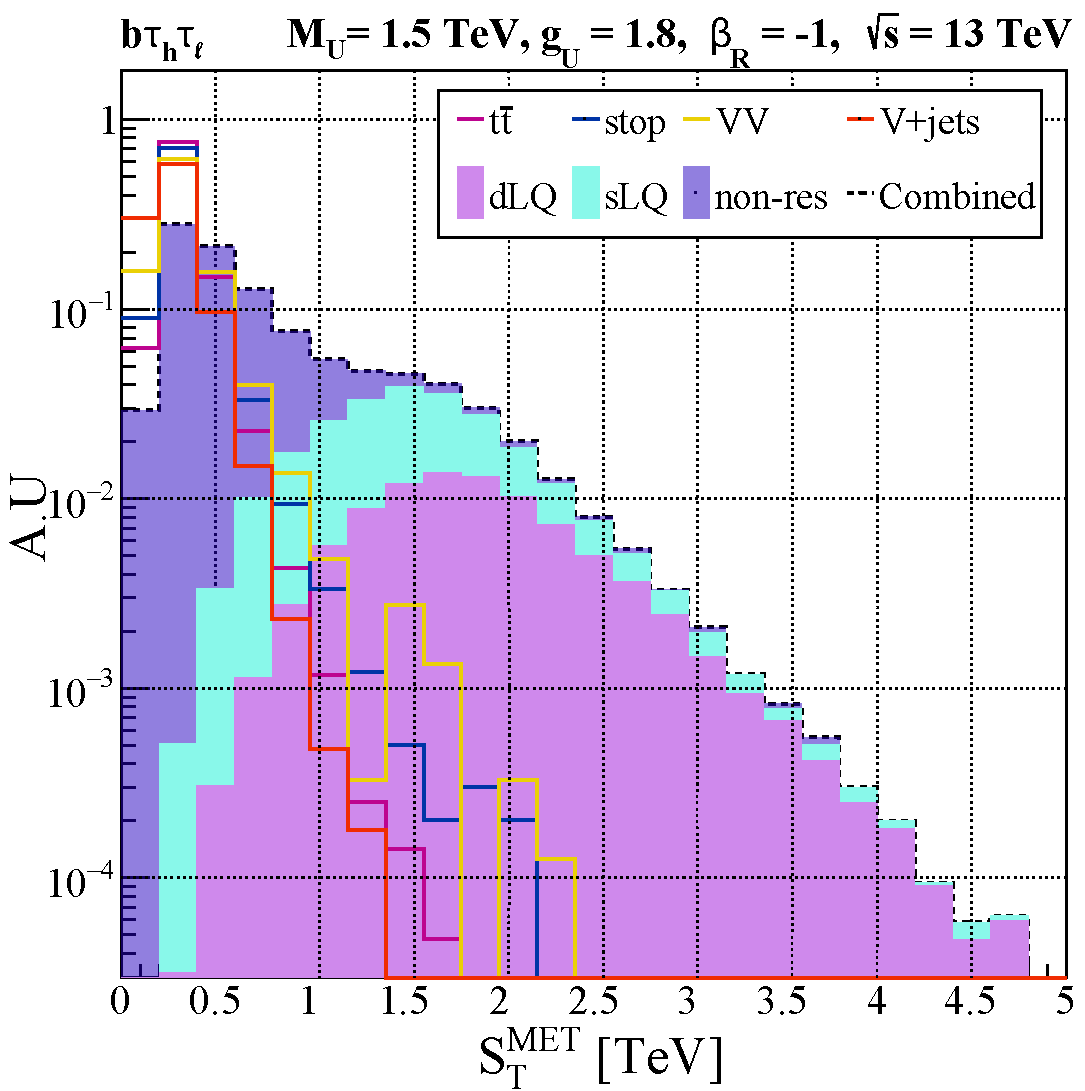
\includegraphics[width=.45\textwidth]{Images/Kinematic_Histograms/sTTeV_semileptonic_sLQ_wRHC.pdf}
    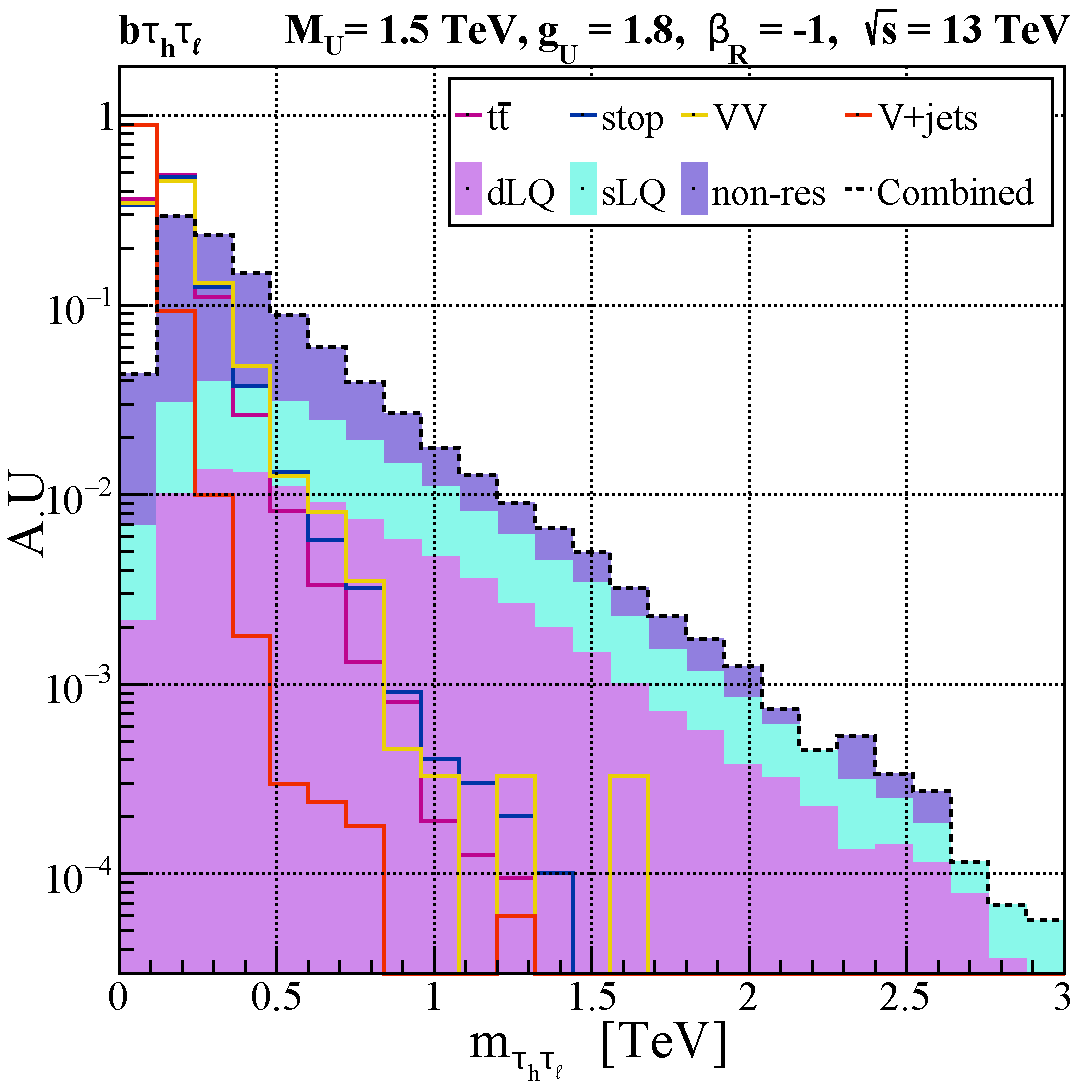
\includegraphics[width=.45\textwidth]{Images/Kinematic_Histograms/mTeV_semileptonic_sLQ_wRHC.pdf}
    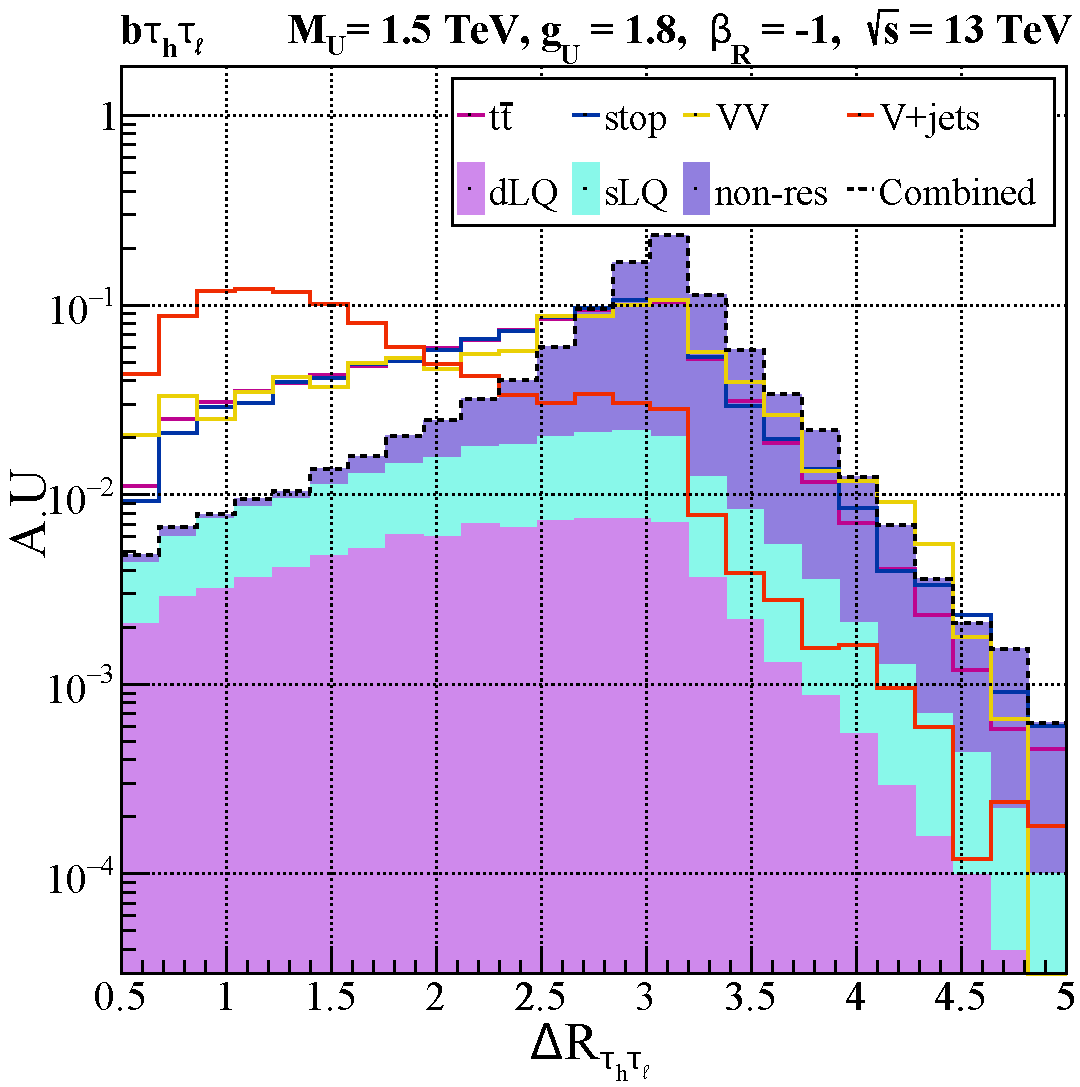
\includegraphics[width=.45\textwidth]{Images/Kinematic_Histograms/DeltaR_semileptonic_sLQ_wRHC.pdf}
    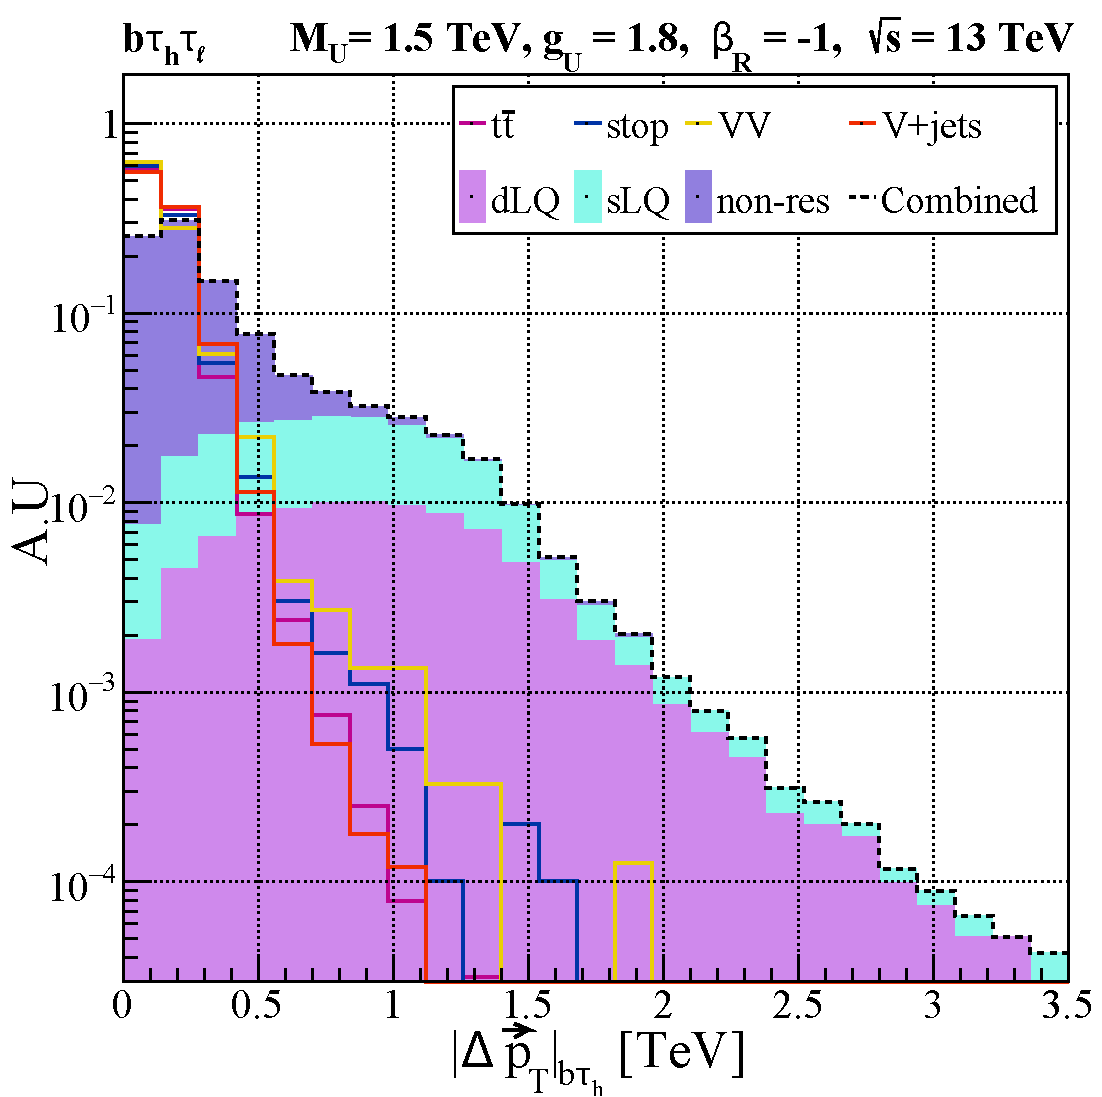
\includegraphics[width=.45\textwidth]{Images/Kinematic_Histograms/DeltaVecPT_semileptonic_sLQ_wRHC.pdf}    
    \captionof{figure}{$S_{\mathrm{T}}^{MET}$, $m_{\tau_{\mathrm h} \tau_{\ell}}$, $\Delta R_{\tau_{\mathrm h}\tau_{\ell}}$, $|\Delta \vec{p}_T|_{b \tau_{\mathrm h}}$ signal and background distributions for the $b\tau_h\tau_\ell$ channel. The signal distributions are generated for a benchmark sample with $\lq$ mass of $1.5 \tev$  maximally coupled to right-handed currents. The combined distribution (shown as a stacked histogram) is the sum of the distributions, correctly weighted according to their respective cross-sections, assuming a coupling $g_U = 1.8$.}
    \label{fig:sT(TeV)_wRHC}
\end{center}




Figure~\ref{fig:sT(TeV)_wRHC} shows some relevant topological distributions, including $S_{\mathrm{T}}^{MET}$ on the top, for the $\bq\, \tau_{\mathrm h} \tau_{\ell}$ category.  
In the Figure we include all signal production modes to this channel, with each component weighted with respect to their total contribution to the combined signal. The combined signal distribution is normalised to unity. We also show all background processes contributing to this channel, each of them individually normalised to unity. We find that the combined signal is dominated by s$\lq$ production for large values of $S_{\mathrm{T}}^{MET}$, while non-res production dominates for small $S_{\mathrm{T}}^{MET}$. Interestingly, the backgrounds also sit at low $S_{\mathrm{T}}^{MET}$ values, since $S_{\mathrm{T}}^{MET}$ is driven by the mass scale of the SM particles being produced, in this case top quarks and Z/W bosons. This suggest that the s$\lq$ and d$\lq$ signals can indeed be separated from the SM background. As expected, the $S_{\mathrm{T}}^{MET}$ s$\lq$ and d$\lq$ signal distributions have a mean near $M_U$, representative of resonant production, and a broad width as expected for large mass $M_{U}$ hypotheses when information about the $z$-components of the momenta of objects is not utilised in the $S_{\mathrm{T}}^{MET}$ calculation.  

Figure~\ref{fig:sT(TeV)_wRHC} (second from the top) shows the reconstructed mass of the ditau system, for the $\bq \tau_{\textrm{h}}\tau_{\ell}$ search channel. Since the two $\tau$ candidates in signal events arise from different production vertices (e.g., each $\tau$ candidate in d$\lq$ production comes from a different $\lq$ decay chain), the ditau mass distribution for signal scales as $m_{\tau_{\textrm{h}}\tau_{\ell}} \sim \pt(\tau_{\textrm{h}}) + \pt(\tau_{\ell})$, and thus has a tail which depends on $M_{U}$ and sits above the expected SM spectrum. On the other hand, the SM $m_{\tau_{\textrm{h}}\tau_{\ell}}$ distributions sit near $m_{\textrm{Z/W}}$ since the $\tau$ candidates in SM events arise from $\zb/\wb$ decays.

Figure~\ref{fig:sT(TeV)_wRHC} (third from the top) shows the $\Delta R_{\tau_{\textrm{h}}\tau_{\ell}}$ distribution for the $\textrm{b}\tau_{\textrm{h}}\tau_{\ell}$ channel. In the case of the $\mathrm{p}\,\mathrm{p}\to\tau\tau$ non-res signal distribution, the two $\tau$ leptons must be back-to-back to preserve conservation of momentum. Therefore, the visible $\tau$ candidates, $\tau_{\textrm{h}}$ and $\tau_{\ell}$, give rise to a $\Delta R_{\tau_{\textrm{h}}\tau_{\ell}}$ distribution that peaks near $\pi$ radians. In the case of s$\lq$ production, although the $\lq$ and associated $\tau$ candidate must be back-to-back, the second $\tau$ candidate arising directly from the decay of the $\lq$ does not necessarily move along the direction of the $\lq$ (since the $\lq$ also decays to a b quark). As a result, the $\Delta R_{\tau_{\textrm{h}}\tau_{\ell}}$ distribution for the s$\lq$ signal process is smeared out, is broader, and has a mean below $\pi$ radians. On the other hand, the $\tau_{\textrm{h}}$ candidate in $\tq\bar{ \tq}$ events is often a jet being misidentified as a genuine $\tau_{\textrm{h}}$. When this occurs, the fake $\tau_{\textrm{h}}$ candidate can arise from the same top quark decay chain as the $\tau_{\ell}$ candidate, thus giving rise to small $\Delta R_{\tau_{\textrm{h}}\tau_{\ell}}$ values. This difference in the signal and background distributions provides a nice way for the ML algorithm to help decipher signal and background processes.

As noted above, the $|\Delta \vec{p}_{T}|$ distribution between the visible $\tau$ candidates and the b-quark jets is an important variable to help the BDT distinguish between signal and background processes. The discriminating power can be seen in Figure~\ref{fig:sT(TeV)_wRHC} (bottom), which shows the $|\Delta \vec{p}_{T}|$ between the $\tau_{\textrm{h}}$ and b-jet candidate of the $\textrm{b}\tau_{\textrm{h}}\tau_{\ell}$ channel. In the case of d$\lq$ production, the b quarks and $\tau$ leptons from the $\lq \to \textrm{b}\tau$ decay acquire transverse momentum of $p_{T} \sim M_{U}/2$. However, when the $\tau$ lepton decays hadronically (i.e. $\tau \to \tau_{\textrm{h}}\nu$), a large fraction of the momentum is lost to the neutrino. Therefore, the $|\Delta \vec{p}_{T}|_{\textrm{b}\tau_{\textrm{h}}}$ distribution for the d$\lq$ (and s$\lq$) process peaks below $M_{U}$/2. On the other hand, for a background process such as V+jets, the b jet arises due to initial state radiation, and thus must balance the momentum of the associated vector boson (i.e. $p_{T}(\textrm{b}) \sim p_{T}(\textrm{V}) \sim m_{\textrm{V}}$). Since the visible $\tau$ candidate is tyically produced from the V boson decay chain, its momentum (on average) is approximately $p_{T}(\tau_{\textrm{h}}) \sim p_{T}(\textrm{V})/4 \sim m_{\textrm{V}}/4$. Therefore, to first order, the $|\Delta \vec{p}_{T}|$ distribution for the V+jets background is expected to peak below the $m_{\textrm{V}}$ mass. 

\begin{figure}[]
    \centering
    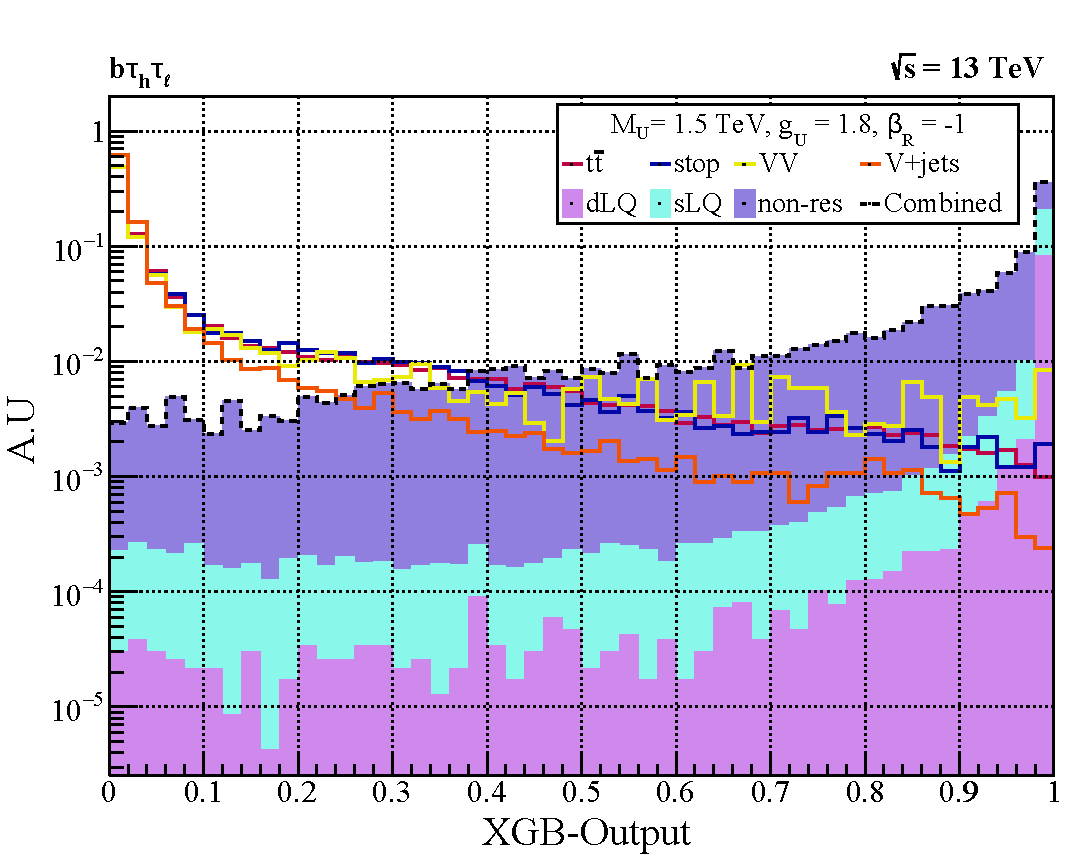
\includegraphics[width=.75\linewidth]{Images/ML_semileptonic_sLQ_wRHC.pdf}
    \caption{Postfit XGB-output normalised distribution in the $\bq\, \tau_{\mathrm h} \tau_{\ell}$ channel, for $\lq$ mass of 1.5\tev, constant coupling $g_U=1.8$, and maximally coupled to right-handed currents.}
    \label{fig:XGB_output}
\end{figure}
Lets us turn to the results of the $\bq\tau_{\mathrm h}\tau_\ell$ BDT classifier, which is shown in Figure~\ref{fig:XGB_output} for the different signal production modes and backgrounds. Similar to Figure~\ref{fig:sT(TeV)_wRHC}, the distribution for each individual signal production mode is weighted with respect to their total contribution to the combined signal. The background distributions and combined signal distribution are normalized to an area under the curve of unity. Figure~\ref{fig:XGB_output} shows the XGB distributions for a signal benchmark point with $M_{U} = 1.5$ TeV, $g_{U} = 1.8$, and $\beta_{R} = -1$. The XGB output is a value between 0 and 1, which quantifies the likelihood that an event is either signal-like (XGB output near 1) or background-like (XGB output near 0). We see that the presence of the s$\lq$ and d$\lq$ production modes is observed as an enhancement near a XGB output of unity, while the backgrounds dominate over the low end of the XGB output spectrum, especially near zero. In fact, over eighty percent of the sLQ and dLQ distributions reside in the last two bins, XGB output greater than 0.96, while more than sixty percent of the backgrounds fall in the first two bins, XGB output less than 0.04. %\JPP{23\% lie on the left of XGB = 0.7}.
It is also interesting to note that in comparison to the sLQ and dLQ distributions in Figure~\ref{fig:XGB_output}, non-res is broader and not as narrowly peaked near XGB output of 1, which is expected due to the differences in kinematics described above. Overall, if we focus on the last bin in this distribution, we find approximately 0.2\% of the background, in contrast to 22\% of the non-res, 78\% of the sLQ, and 91\% of the dLQ signal distributions. These numbers highlight the effectiveness of the XGB output in reducing the background in the region where the signal is expected.

The output signal and background distributions of the XGB classifier, normalised to their cross section times pre-selection efficiency times luminosity, are used to perform a profile binned likelihood statistical test in order to determine the expected signal significance. The estimation is performed using the \texttt{RooFit}~\cite{RooFit} package, following the same methodology as in Refs.~\cite{Barbosa:2022mmw, Florez:2021zoo, Florez:2019tqr, Florez:2018ojp, Florez:2017xhf, VBFZprimePaper, Florez:2016lwi, U1T3R, mSUGRApaper, SupercriticalString, ConnectingPPandCosmology, VBF1, DMmodels2, VBFSlepton, VBFStop, VBFSbottom}. The value of the significance ($Z_{sig}$) is measured using the probability to obtain the same outcome from the test statistic in the background-only hypothesis, with respect to the signal plus background hypothesis. This allows for the determination of the local p-value and thus the calculation of the signal significance, which corresponds to the point where the integral of a Gaussian distribution between $Z_{sig}$ and $\infty$ results in a value equal to the local p-value. 

Systematic uncertainties are incorporated as nuisance parameters, considering log-priors for normalization and Gaussian priors for shape uncertainties. Our consideration of systematic uncertainties includes both experimental and theoretical effects, focusing on the dominant sources of uncertainty. Following~\cite{lumiRef}, we consider a 3\% systematic uncertainty on the measurement of the integrated luminosity at the LHC. A 5\% uncertainty arises due to the choice of the parton distribution function used for the MC production, following the PDF4LHC prescription~\cite{Butterworth:2015oua}. The chosen PDF set only has an effect on the overall expected signal and background yields, but the effect on the shape of the XGB output distribution is negligible. Reference~\cite{CMS_DeepTau} reports a systematic uncertainty of 2-5\%, depending on the $p_{\textrm{T}}$ and $\eta$ of the $\tau_{\textrm{h}}$ candidate. Therefore, we utilize a conservative 5\% uncertainty per $\tau_{\textrm{h}}$ candidate, independent of $p_{\textrm{T}}$ and $\eta$, which is correlated between signal and background processes with genuine $\tau_{\textrm{h}}$ candidates, and correlated across XGB bins for each process. We assumed a 5\% $\tau_{\textrm{h}}$ energy scale uncertainty, independent of $p_{\textrm{T}}$ and $\eta$, following the CMS measurements described in~\cite{CMS_DeepTau}.  Finally, we assume a conservative 3\% uncertainty per b-jet candidate, following reference~\cite{CMSbtag}, and an additional 10\% uncertainty in all the background predictions to account for possible mismodeling by the simulated samples. The uncertainties on the background estimates are typically derived from collision data using dedicated control samples that have negligible signal contamination and are enriched with events from the specific targeted background. The systematic uncertainties on the background estimates are treated as uncorrelated between background processes.
\begin{figure}[]
    \centering
        \begin{subfigure}[b]{.48\linewidth}
            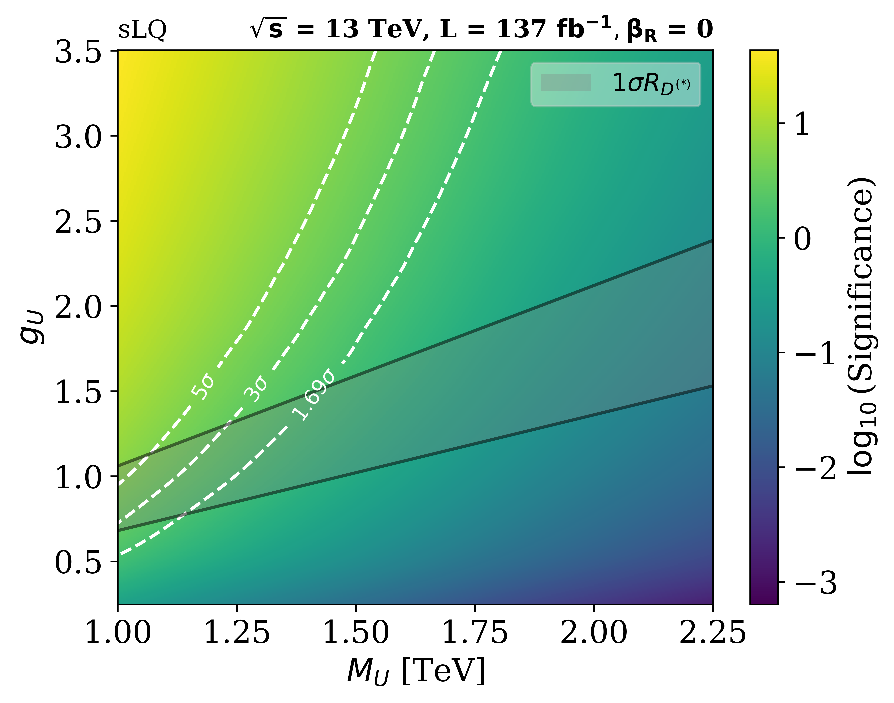
\includegraphics[width=\linewidth]{Images/Significance/Significance_Heatmap_13TeV_L137_sLQ_combined_woRHC.pdf}
        \end{subfigure}
        \begin{subfigure}[b]{.48\linewidth}
            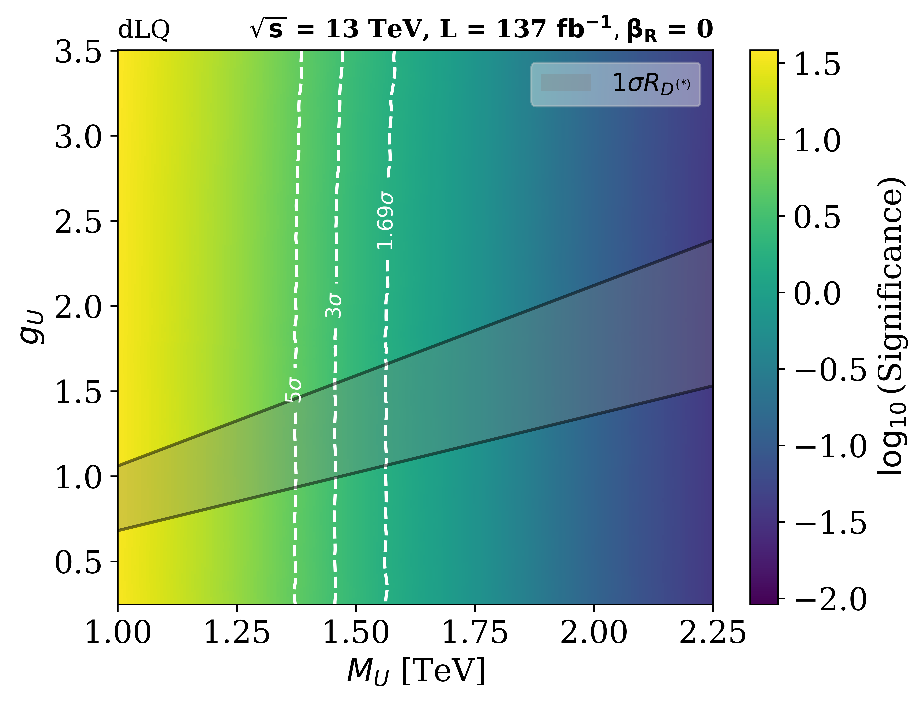
\includegraphics[width=\linewidth]{Images/Significance/Significance_Heatmap_13TeV_L137_dLQ_combined_woRHC.pdf}
        \end{subfigure}     
        \begin{subfigure}[b]{.48\linewidth}
            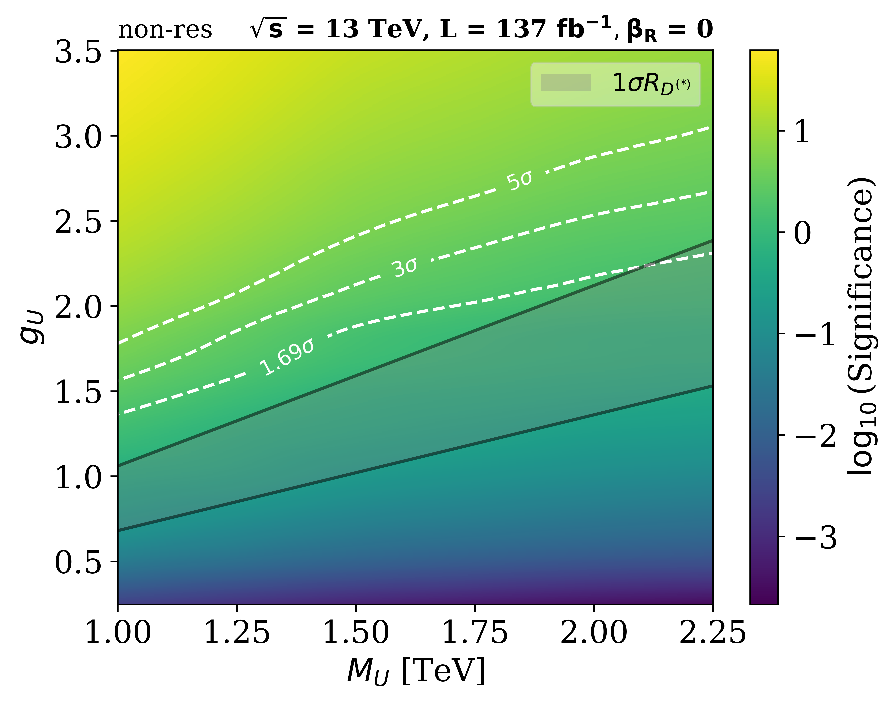
\includegraphics[width=\linewidth]{Images/Significance/Significance_Heatmap_13TeV_L137_non-res_combined_woRHC.pdf}
        \end{subfigure}    
 
    \caption{Signal significance for different coupling scenarios and $\lq$ masses, without right-handed currents, using the combination of all search channels. The results pertaining to  s$\lq$, d$\lq$ and non-res production are displayed respectively from the top.  These results are for $\sqrt{s} = 13 \tev$ and $137 \fb^{-1}$.}
    \label{fig:heatmapssignificance}
\end{figure}